\section{Fase 1: BCQM} 
En esta fase se propone el uso de un mapa de preguntas sobre el cáncer de mama (Por sus siglas en ingles Breast Cancer Question Map (BCQM)). El proposito del \textit{BCQM} es que el \textit{Data Analysis Team} defina las preguntas que serán resueltas al finalizar cada \textit{Release} y que permitirán tomar decisiones medicas con respecto al diagnostico de esta enfermedad. En la figura \ref{BCQM} se observa la estructura del BCQM.

\begin{figure}
	\centering
	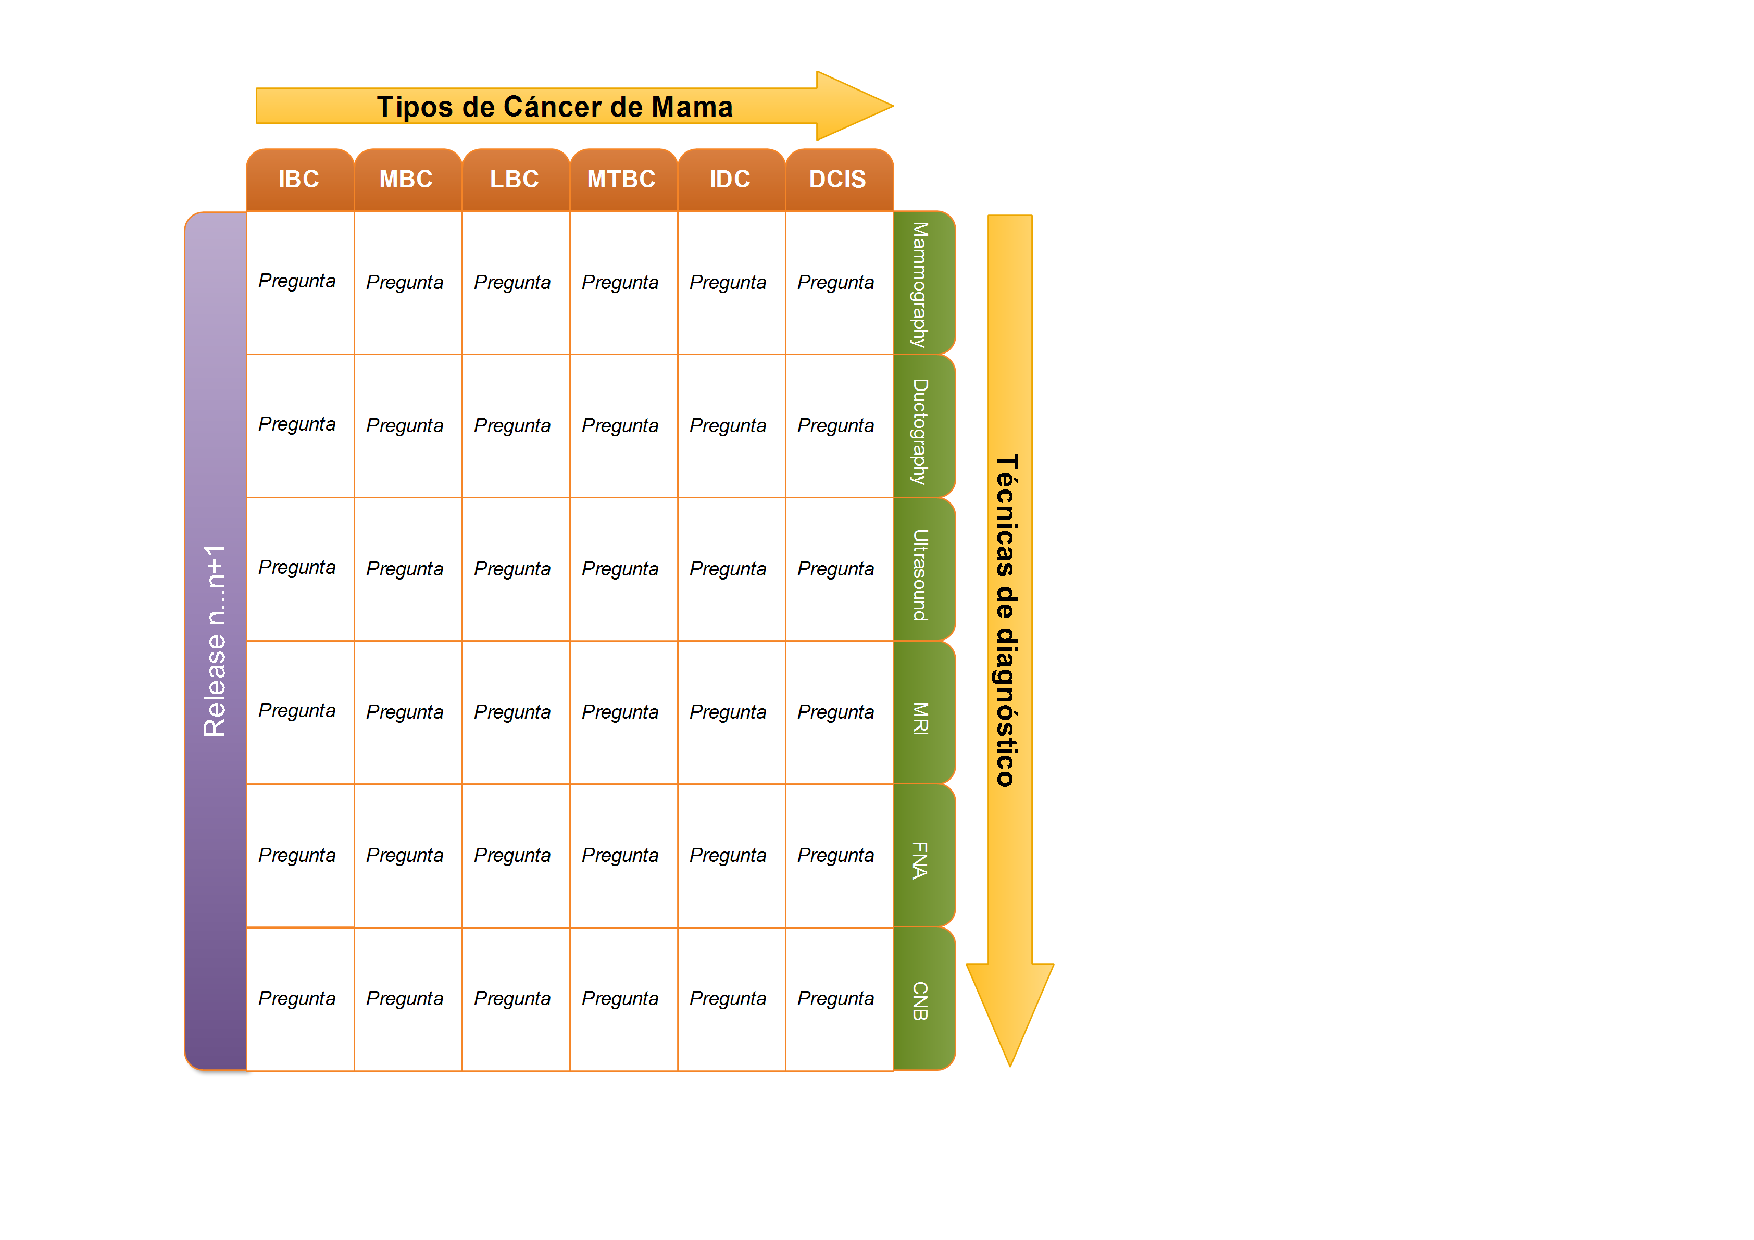
\includegraphics[width=0.8
	\linewidth]{IMAGENES/BCQM_SPANISH}
	\caption{Breast Cancer Question Map (BCQM). Aplicado a tipos de cáncer \textit{Inflamatorio (IBC)}, \textit{mucinoso (MBC)}, \textit{Lobulillar (LBC)}, \textit{Tumores mixtos (MTBC)}, \textit{Carcinoma ductal invasivo (IDC)} y \textit{Carcinoma ductal in situ (DCIS)}}
	\label{BCQM}
\end{figure}

El BCQM permite plantear preguntas relacionadas a los tipos de cáncer de mama y a las técnicas para el diagnostico de la misma. De modo que al finalizar el tiempo de cada \textit{Release}, el cual puede variar entre 1 y 4 semanas, las preguntas serán respondidas según el análisis de datos generado, y el medico podrá tomar una decisión de valor. Cabe resaltar, que es posible tener una o mas preguntas relacionadas a una técnica y a un tipo de cáncer de mama por cada \textit{Release}, razón por la cual es posible encontrar correlaciones entre las variables características de cada tipo de cáncer encontrando así patrones ocultos en los diferentes conjuntos de datos.

 Con base a lo anterior, es recomendable que se generen máximo 3 preguntas por Release, debido a que a nivel de ciencia de datos la respuesta de una sola pregunta conlleva a un proceso complejo y el objetivo principal de la metodología es generar respuestas de valor que aporten en la agilidad del diagnostico del cáncer de mama, por lo que generar una cantidad muy grande de preguntas puede generar un desperdicio de informacion en el tiempo establecido en el Release para dar una respuesta.
 
 Adicionalmente, el BCQM permite identificar a que técnica para el diagnostico de cáncer mama esta relacionada la pregunta a resolver, lo cual de antemano hace posible conocer el tipo información (imágenes o datos) y el algoritmo  ML o DL requerido para dar solución al problema. Dada la naturaleza de las preguntas, es posible  que las mismas estén relacionadas a varias técnicas de diagnostico al mismo tiempo. Así mismo, el BCQM permite definir desde la fase inicial el tipo de modelo predictivo o descriptivo según el enfoque analítico generado por la pregunta planteada. Sintetizando, el uso de BCQM facilita la comprensión del problema medico y permite identificar previamente la técnica, el tipo de información y enfoque que debe ser utilizado para el análisis de datos.  

Para este caso de estudio, se plantearon las preguntas que observan en la figura \ref{BCQ_TCGA} a partir del proyecto de carcinoma invasivo de mama denominado \textit{“Comprehensive Molecular Portraits of Invasive Lobular Breast Cancer”}\cite{Ciriello2015}, basado en el \textit {Atlas del Genoma del Cáncer (TCGA\footnote{Acrónimo de “The Cancer Genome Atlas (TCGA)”, en inglés })} cuya finalidad es catalogar cambios moleculares de importancia biológica responsables de la aparición de cáncer haciendo uso de la secuenciación genómica y la bioinformática \cite{TCGA2023}.
\begin{figure}
	\centering
	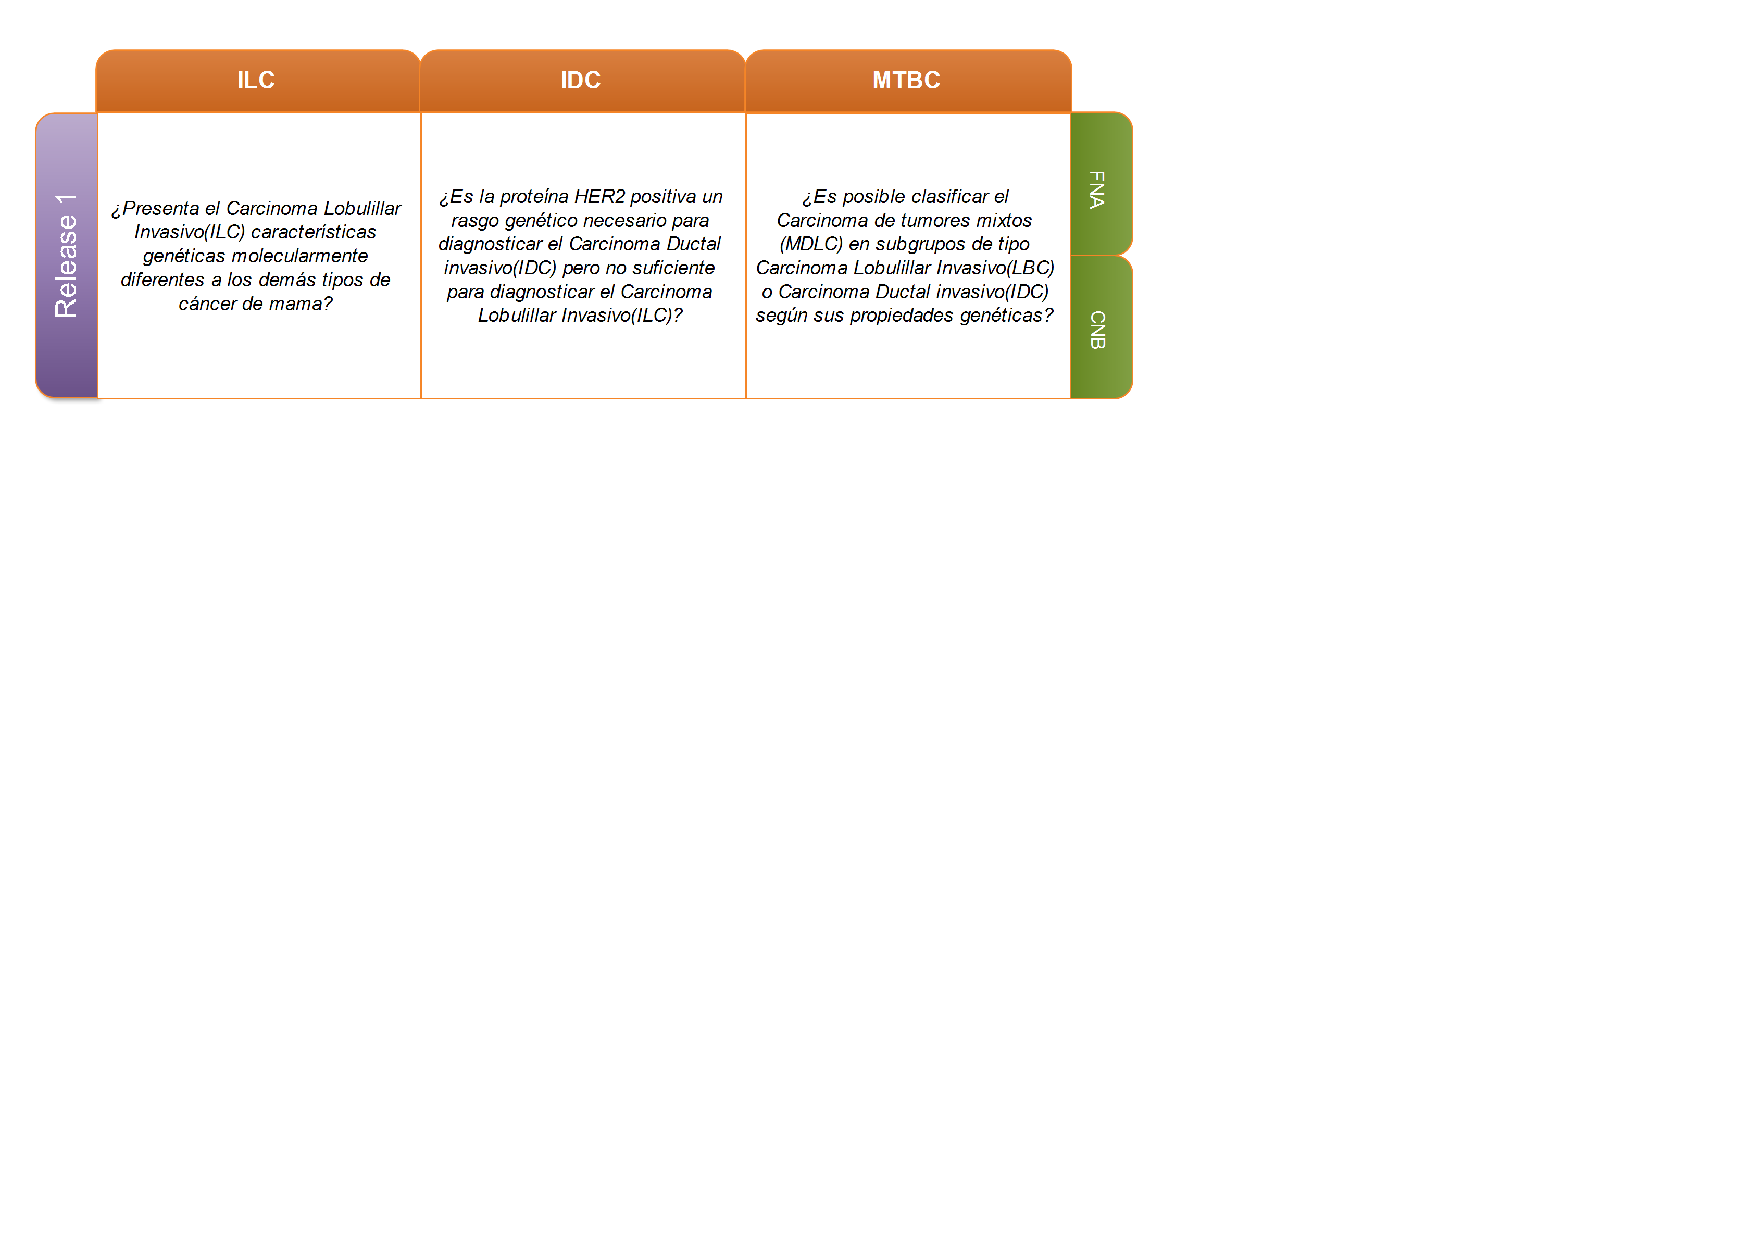
\includegraphics[width=1
	\linewidth]{IMAGENES/BCQM_TCGA}
	\caption{BCQM generado para el caso de estudio.}
	\label{BCQ_TCGA}
\end{figure}

Dadas las preguntas generadas, los tipos de cáncer de mama seleccionados son los siguientes:
\begin{itemize}[label=\HandRight]
	\item \textbf{Carcinoma Lobulillar Invasivo (LBC)}:  Este tipo de cáncer ocurre dentro del lóbulo mamario y aumenta las posibilidades de otros cánceres invasivos. 
	\item \textbf{Carcinoma Ductal Invasivo (IDC)}:Este tipo de cáncer ocurre cuando las células anormales de la mama se diseminan por los conductos conformados por los tejidos mamarios.
	\item \textbf{Tumores Mixtos (MTBC)}: Este tipo de cáncer es causado por las células anormales de los conductos y las células lobulillares, por que esta conformado por los tipos de cáncer LBC e IDC.
\end{itemize}

Con base a los tipos de cáncer de mama anteriores y a las preguntas planteadas en el BCQM que requieren informacion de índole genético, la técnica de diagnóstico mas adecuada es la \textit{Biopsia}. Dado lo anterior, en el BCQM se relacionan las biopsias que incluyen las siguientes técnicas: 

\begin{itemize}[label=\HandRight]
	\item \textbf{Biopsia por aspiración con aguja fina (FNA\footnote{Fine Needle Aspiration})}: Se usa una aguja calibre 22 de 4 cm unida a una jeringa de 10 ml. El uso de un soporte de la jeringa permite que el cirujano que toma la biopsia controle la jeringa y la aguja con una mano en tanto sitúa la masa mamaria con la mano opuesta. Tras colocar la aguja en la masa, se aspira en tanto se mueve la aguja hacia adelante y atrás dentro de la masa. La aspiración se detiene y la aguja se extrae una vez que se observa material celular en la cabeza de la aguja \cite{Brunicardi2010}. Este procedimiento quirúrgico se puede observar en la figura \ref{FNB}.
	 \begin{figure}[!htb]
	 	\centering
	 	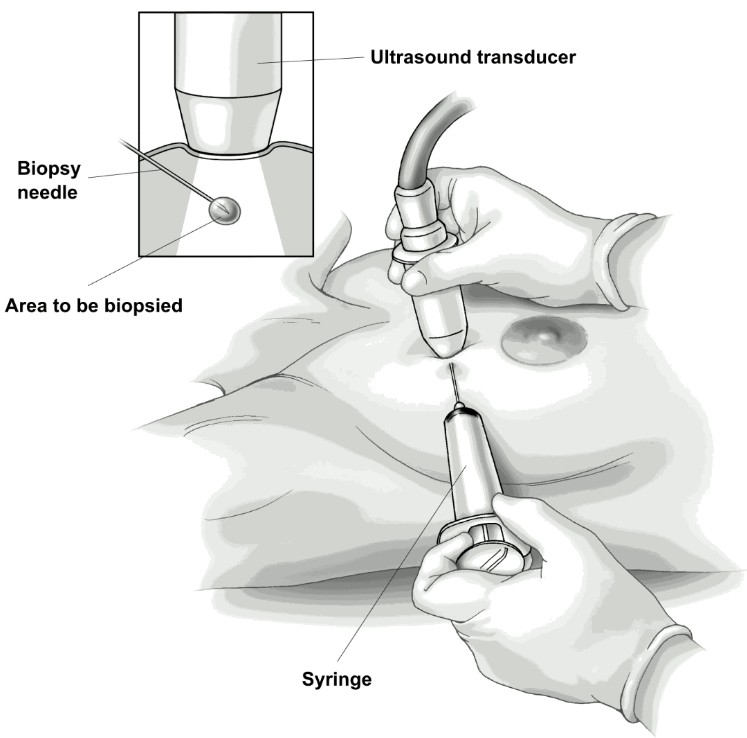
\includegraphics[width=0.5
	 	\linewidth]{IMAGENES/FNB}
	 	\caption{Aspiración con aguja fina\cite{FNB}.}
	 	\label{FNB}
	 \end{figure}	
	 \\
	
	\item \textbf{Biopsia con aguja gruesa (CNB\footnote{Core Needle Biopsy})}: Se usa en masas palpables de la mama  con una aguja calibre 14, como la Tru-Cut. También se cuenta con dispositivos automatizados. Las muestras de tejidos se colocan en formalina y luego se procesan para bloques de parafina \cite{Brunicardi2010}. Este procedimiento quirúrgico se puede observar en la figura \ref{CNB}.
	\begin{figure}[!htb]
		\centering
		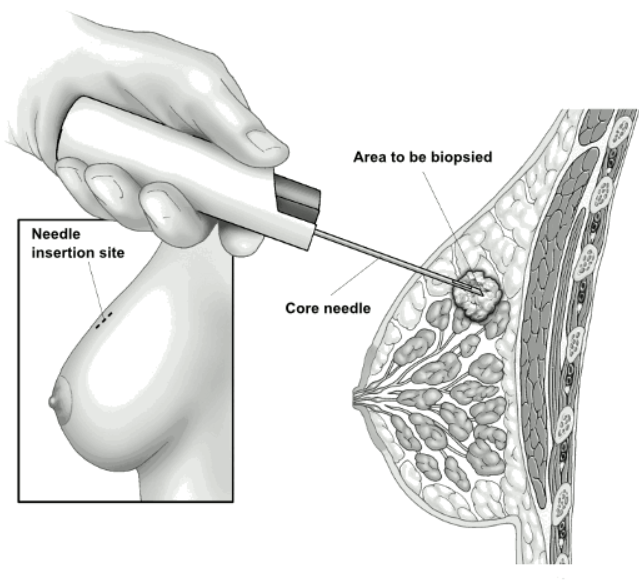
\includegraphics[width=0.5
		\linewidth]{IMAGENES/CNB}
		\caption{Biopsia con aguja gruesa\cite{CNB}.}
		\label{CNB}
	\end{figure}	
\end{itemize}

Considerando la naturaleza de la información, la técnica computacional a utilizar es \textit{Machine Learning} debido a que los datos son de origen genómico y por ende tendrán una representación simbólica con atributos cuantitativos y/o cualitativos. Cabe resaltar, que dado el origen de las preguntas, los modelos de ML a utilizar deben permitir realizar los siguientes tipos de análisis:

\begin{itemize}[label=\HandRight]
	\item \textbf{Análisis Descriptivo}:
	Este tipo de análisis se genera a partir de datos de entrada que no están etiquetados y no tienen un resultado conocido \cite{JorgeCalvo2020}.
	
	\item \textbf{Análisis Predictivo}:Este tipo de análisis se genera a partir de datos históricos reales para hacer predicciones acerca del valor de una variable o dato desconocido \cite{JorgeCalvo2020}.
\end{itemize}

